\documentclass{standalone}
\usepackage{tikz}
\usetikzlibrary{patterns, positioning}

\begin{document}
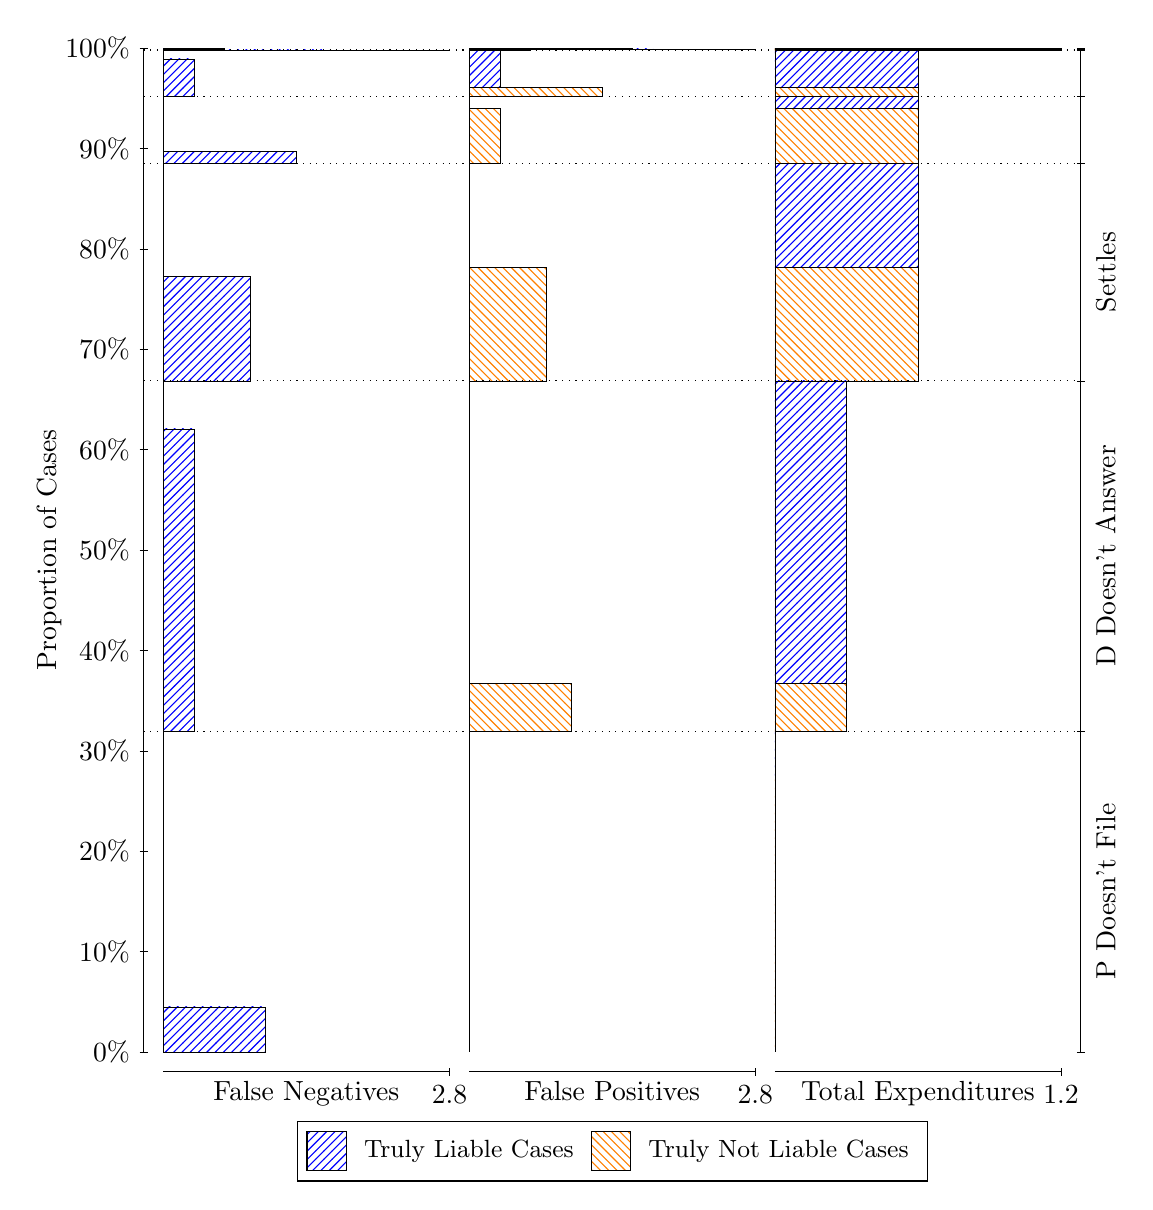
\begin{tikzpicture}
\draw[black, very thin] (1.5,1.75) -- (1.5,14.5);
\node[rotate=90, anchor=center] at (0.3, 8.125) {Proportion of Cases};
\draw[black, very thin] (1.45,1.75) -- (1.55,1.75);
\node[anchor=east] at (1.45, 1.75) {0\%};
\draw[black, very thin] (1.45,3.025) -- (1.55,3.025);
\node[anchor=east] at (1.45, 3.025) {10\%};
\draw[black, very thin] (1.45,4.3) -- (1.55,4.3);
\node[anchor=east] at (1.45, 4.3) {20\%};
\draw[black, very thin] (1.45,5.575) -- (1.55,5.575);
\node[anchor=east] at (1.45, 5.575) {30\%};
\draw[black, very thin] (1.45,6.85) -- (1.55,6.85);
\node[anchor=east] at (1.45, 6.85) {40\%};
\draw[black, very thin] (1.45,8.125) -- (1.55,8.125);
\node[anchor=east] at (1.45, 8.125) {50\%};
\draw[black, very thin] (1.45,9.4) -- (1.55,9.4);
\node[anchor=east] at (1.45, 9.4) {60\%};
\draw[black, very thin] (1.45,10.675) -- (1.55,10.675);
\node[anchor=east] at (1.45, 10.675) {70\%};
\draw[black, very thin] (1.45,11.95) -- (1.55,11.95);
\node[anchor=east] at (1.45, 11.95) {80\%};
\draw[black, very thin] (1.45,13.225) -- (1.55,13.225);
\node[anchor=east] at (1.45, 13.225) {90\%};
\draw[black, very thin] (1.45,14.5) -- (1.55,14.5);
\node[anchor=east] at (1.45, 14.5) {100\%};

\draw[black, very thin] (13.4,1.75) -- (13.4,14.5);
\draw[black, very thin] (13.35,1.75) -- (13.45,1.75);
\node[anchor=west] at (13.35, 1.75) {};
\draw[black, very thin] (13.35,5.825) -- (13.45,5.825);
\node[anchor=west] at (13.35, 5.825) {};
\draw[black, very thin] (13.35,10.274) -- (13.45,10.274);
\node[anchor=west] at (13.35, 10.274) {};
\draw[black, very thin] (13.35,13.038) -- (13.45,13.038);
\node[anchor=west] at (13.35, 13.038) {};
\draw[black, very thin] (13.35,13.885) -- (13.45,13.885);
\node[anchor=west] at (13.35, 13.885) {};
\draw[black, very thin] (13.35,14.472) -- (13.45,14.472);
\node[anchor=west] at (13.35, 14.472) {};
\draw[black, very thin] (13.35,14.486) -- (13.45,14.486);
\node[anchor=west] at (13.35, 14.486) {};
\draw[black, very thin] (13.35,14.5) -- (13.45,14.5);
\node[anchor=west] at (13.35, 14.5) {};

\draw[black, very thin, pattern color=blue, pattern=north east lines] (1.75,1.75) rectangle (3.0476,2.3219);
\draw[black, very thin, pattern color=orange, pattern=north west lines] (1.75,2.3219) rectangle (1.75,5.825);
\draw[black, very thin, pattern color=blue, pattern=north east lines] (1.75,5.825) rectangle (2.1393,9.6634);
\draw[black, very thin, pattern color=orange, pattern=north west lines] (1.75,9.6634) rectangle (1.75,10.274);
\draw[black, very thin, pattern color=blue, pattern=north east lines] (1.75,10.274) rectangle (2.853,11.595);
\draw[black, very thin, pattern color=orange, pattern=north west lines] (1.75,11.595) rectangle (1.75,13.038);
\draw[black, very thin, pattern color=blue, pattern=north east lines] (1.75,13.038) rectangle (3.4369,13.191);
\draw[black, very thin, pattern color=orange, pattern=north west lines] (1.75,13.191) rectangle (1.75,13.885);
\draw[black, very thin, pattern color=blue, pattern=north east lines] (1.75,13.885) rectangle (2.1393,14.362);
\draw[black, very thin, pattern color=orange, pattern=north west lines] (1.75,14.362) rectangle (1.75,14.472);
\draw[black, very thin, pattern color=blue, pattern=north east lines] (1.75,14.472) rectangle (5.3833,14.473);
\draw[black, very thin, pattern color=blue, pattern=north east lines] (1.75,14.473) rectangle (3.8262,14.477);
\draw[black, very thin, pattern color=orange, pattern=north west lines] (1.75,14.477) rectangle (1.75,14.486);
\draw[black, very thin, pattern color=blue, pattern=north east lines] (1.75,14.486) rectangle (2.5286,14.492);
\draw[black, very thin, pattern color=orange, pattern=north west lines] (1.75,14.492) rectangle (1.75,14.497);
\draw[black, very thin, pattern color=blue, pattern=north east lines] (1.75,14.497) rectangle (1.75,14.5);
\draw[black, very thin, pattern color=orange, pattern=north west lines] (5.6333,1.75) rectangle (5.6333,5.2531);
\draw[black, very thin, pattern color=blue, pattern=north east lines] (5.6333,5.2531) rectangle (5.6333,5.825);
\draw[black, very thin, pattern color=orange, pattern=north west lines] (5.6333,5.825) rectangle (6.931,6.4358);
\draw[black, very thin, pattern color=blue, pattern=north east lines] (5.6333,6.4358) rectangle (5.6333,10.274);
\draw[black, very thin, pattern color=orange, pattern=north west lines] (5.6333,10.274) rectangle (6.6065,11.717);
\draw[black, very thin, pattern color=blue, pattern=north east lines] (5.6333,11.717) rectangle (5.6333,13.038);
\draw[black, very thin, pattern color=orange, pattern=north west lines] (5.6333,13.038) rectangle (6.0226,13.732);
\draw[black, very thin, pattern color=blue, pattern=north east lines] (5.6333,13.732) rectangle (5.6333,13.885);
\draw[black, very thin, pattern color=orange, pattern=north west lines] (5.6333,13.885) rectangle (7.3202,13.996);
\draw[black, very thin, pattern color=blue, pattern=north east lines] (5.6333,13.996) rectangle (6.0226,14.472);
\draw[black, very thin, pattern color=orange, pattern=north west lines] (5.6333,14.472) rectangle (6.4119,14.478);
\draw[black, very thin, pattern color=orange, pattern=north west lines] (5.6333,14.478) rectangle (5.6333,14.481);
\draw[black, very thin, pattern color=blue, pattern=north east lines] (5.6333,14.481) rectangle (5.6333,14.486);
\draw[black, very thin, pattern color=orange, pattern=north west lines] (5.6333,14.486) rectangle (9.2667,14.486);
\draw[black, very thin, pattern color=blue, pattern=north east lines] (5.6333,14.486) rectangle (7.969,14.489);
\draw[black, very thin, pattern color=orange, pattern=north west lines] (5.6333,14.489) rectangle (7.7095,14.493);
\draw[black, very thin, pattern color=blue, pattern=north east lines] (5.6333,14.493) rectangle (6.4119,14.5);
\draw[black, very thin, pattern color=orange, pattern=north west lines] (9.5167,1.75) rectangle (9.5167,5.2531);
\draw[black, very thin, pattern color=blue, pattern=north east lines] (9.5167,5.2531) rectangle (9.5167,5.825);
\draw[black, very thin, pattern color=orange, pattern=north west lines] (9.5167,5.825) rectangle (10.425,6.4358);
\draw[black, very thin, pattern color=blue, pattern=north east lines] (9.5167,6.4358) rectangle (10.425,10.274);
\draw[black, very thin, pattern color=orange, pattern=north west lines] (9.5167,10.274) rectangle (11.333,11.717);
\draw[black, very thin, pattern color=blue, pattern=north east lines] (9.5167,11.717) rectangle (11.333,13.038);
\draw[black, very thin, pattern color=orange, pattern=north west lines] (9.5167,13.038) rectangle (11.333,13.732);
\draw[black, very thin, pattern color=blue, pattern=north east lines] (9.5167,13.732) rectangle (11.333,13.885);
\draw[black, very thin, pattern color=orange, pattern=north west lines] (9.5167,13.885) rectangle (11.333,13.996);
\draw[black, very thin, pattern color=blue, pattern=north east lines] (9.5167,13.996) rectangle (11.333,14.472);
\draw[black, very thin, pattern color=orange, pattern=north west lines] (9.5167,14.472) rectangle (13.15,14.478);
\draw[black, very thin, pattern color=blue, pattern=north east lines] (9.5167,14.478) rectangle (13.15,14.483);
\draw[black, very thin, pattern color=orange, pattern=north west lines] (9.5167,14.483) rectangle (13.15,14.485);
\draw[black, very thin, pattern color=blue, pattern=north east lines] (9.5167,14.485) rectangle (13.15,14.486);
\draw[black, very thin, pattern color=orange, pattern=north west lines] (9.5167,14.486) rectangle (13.15,14.49);
\draw[black, very thin, pattern color=blue, pattern=north east lines] (9.5167,14.49) rectangle (13.15,14.497);
\draw[black, very thin, pattern color=orange, pattern=north west lines] (9.5167,14.497) rectangle (13.15,14.497);
\draw[black, very thin, pattern color=blue, pattern=north east lines] (9.5167,14.497) rectangle (13.15,14.5);
\draw[black, dotted] (1.5,5.825) -- (13.4,5.825);
\draw[black, dotted] (1.5,10.274) -- (13.4,10.274);
\draw[black, dotted] (1.5,13.038) -- (13.4,13.038);
\draw[black, dotted] (1.5,13.885) -- (13.4,13.885);
\draw[black, dotted] (1.5,14.472) -- (13.4,14.472);
\draw[black, dotted] (1.5,14.486) -- (13.4,14.486);
\draw[black, very thin] (1.75,1.5) -- (5.3833,1.5);
\node[anchor=north] at (3.5667, 1.5) {False Negatives};
\draw[black, very thin] (5.3833,1.45) -- (5.3833,1.55);
\node[anchor=north] at (5.3833, 1.45) {2.8};

\draw[black, very thin] (5.6333,1.5) -- (9.2667,1.5);
\node[anchor=north] at (7.45, 1.5) {False Positives};
\draw[black, very thin] (9.2667,1.45) -- (9.2667,1.55);
\node[anchor=north] at (9.2667, 1.45) {2.8};

\draw[black, very thin] (9.5167,1.5) -- (13.15,1.5);
\node[anchor=north] at (11.333, 1.5) {Total Expenditures};
\draw[black, very thin] (13.15,1.45) -- (13.15,1.55);
\node[anchor=north] at (13.15, 1.45) {1.2};

\node[black, centered, rotate=90] at (13.72, 3.7875) {P Doesn't File};
\node[black, centered, rotate=90] at (13.72, 8.0496) {D Doesn't Answer};
\node[black, centered, rotate=90] at (13.72, 11.656) {Settles};





\draw (7.449999999999999,1.5) node[draw=none] (baseCoordinate) {};
\begin{scope}[align=center]
        \matrix[scale=0.5, draw=black, below=0.5cm of baseCoordinate, nodes={draw}, column sep=0.1cm]{
            \node[rectangle, draw, minimum width=0.5cm, minimum height=0.5cm, pattern=north east lines, pattern color=blue] {}; &
            \node[draw=none, font=\small] (B) {Truly Liable Cases}; &
            \node[rectangle, draw, minimum width=0.5cm, minimum height=0.5cm, pattern=north west lines, pattern color=orange] {}; &
            \node[draw=none, font=\small] (B) {Truly Not Liable Cases}; \\
            };
\end{scope}

\end{tikzpicture}
\end{document}